\documentclass[11pt]{article}

\usepackage{amssymb} % see: http://milde.users.sourceforge.net/LUCR/Math/mathpackages/amssymb-symbols.pdf
\usepackage{mathtools} % for extended mathematical symbols and more

% Page properties :
% See : https://tex.stackexchange.com/questions/36085/latex-without-pages
\usepackage{geometry}
\geometry{margin=16mm}


% fix for underlined text not hyphenating :
%\usepackage{soul} % use this
% then replace '\underline{}' with '\ul{}'

% To color text :
% see : https://en.wikibooks.org/wiki/LaTeX/Colors
%\usepackage[dvipsnames]{xcolor} % use this
% then use one of these syntaxes :
% >\textcolor{declared-color}{text}
% >{\color{declared-color} text}

% Input file encoding :
\usepackage[utf8]{inputenc}     % makes accents not shit

% To use images : 
%\usepackage{graphicx} % use this
%\graphicspath{ {./IMG/} } % path midifier for storing images
% to include a picture, type this ('name' is without path or extention) :
% \includegraphics[width=0.5\textwidth]{name}

% Box : % width should be manually set
% \fbox{ \parbox{0.8\textwidth}{ text } }

% Espacement :
% \hfill \vfill
% \vspace{length} \hspace{length} % if ignored, use starred version or { \vspace*{length} }
% \phantom{text} 
% Indentation explicite :
% \indent et \noindent
\usepackage{parskip}

% Fractions :
% \frac{num}{denum}  % small text num/denum
% \dfrac{num}{denum} % normal text num/denum

% Coloring text: % works on text and math modes
% \textcolor{declared-color}{text}
% {\color{declared-color}some text}

% How to use references :
%\usepackage{hyperref} % use this
% use '\hypertarget{some_label}{}', then
% and reference it with '\hyperlink{some_label}{some text}'

% To write prooftrees :
% see : http://www.pirbot.com/mirrors/ctan/macros/latex/contrib/ebproof/ebproof.pdf
%\usepackage{ebproof} % use this


% Verbatim blocks :
%\usepackage{verbatim} % normal verbatim
%\usepackage{fancyvrb} % for fancy boxed varbatims

% Alternatives to l,c,r for tables with fixed width as argument
% https://tex.stackexchange.com/questions/12703/how-to-create-fixed-width-table-columns-with-text-raggedright-centered-raggedlef
% ex : \begin{tabular}{|L{0.2\linewidth}|C{34mm}|} ...
\usepackage{array}
\newcolumntype{L}[1]{>{\raggedright\let\newline\\\arraybackslash\hspace{0pt}}m{#1}}
\newcolumntype{C}[1]{>{\centering\let\newline\\\arraybackslash\hspace{0pt}}m{#1}}
\newcolumntype{R}[1]{>{\raggedleft\let\newline\\\arraybackslash\hspace{0pt}}m{#1}}


% To use images : 
\usepackage{graphicx} % use this
\graphicspath{ {./IMG/} } % path midifier for storing images
% to include a picture, type this ('name' is without path or extention) :
% \includegraphics[width=0.5\textwidth]{name}

% For code
\usepackage{listings}
%\begin{lstlisting}
%Put your code he<re.
%\end{lstlisting}

\usepackage{wasysym}

\usepackage{color}

\definecolor{mylightgray}{rgb}{0.98,0.98,0.98}
\definecolor{mygreen}{rgb}{0,0.6,0}
\definecolor{mygray}{rgb}{0.5,0.5,0.5}
\definecolor{mylightgray}{rgb}{0.8,0.8,0.8}
\definecolor{mymauve}{rgb}{0.58,0,0.82}

\usepackage{xcolor,colortbl}
\newcolumntype{a}{>{\columncolor{mylightgray}}l}

\lstset{ 
	backgroundcolor=\color{mylightgray},   % choose the background color; you must add \usepackage{color} or \usepackage{xcolor}; should come as last argument
	basicstyle=\small,        % the size of the fonts that are used for the code
	breakatwhitespace=false,         % sets if automatic breaks should only happen at whitespace
	breaklines=true,                 % sets automatic line breaking
	captionpos=b,                    % sets the caption-position to bottom
	commentstyle=\color{mygreen},    % comment style
	deletekeywords={...},            % if you want to delete keywords from the given language
	escapeinside={\%*}{*)},          % if you want to add LaTeX within your code
	extendedchars=true,              % lets you use non-ASCII characters; for 8-bits encodings only, does not work with UTF-8
	firstnumber=1,                % start line enumeration with line 1000
	frame=single,	                   % adds a frame around the code
	keepspaces=true,                 % keeps spaces in text, useful for keeping indentation of code (possibly needs columns=flexible)
	keywordstyle=\color{blue},       % keyword style
	%language=Java,                 % the language of the code
	morekeywords={},            % if you want to add more keywords to the set
	numbers=none,                    % where to put the line-numbers; possible values are (none, left, right)
	numbersep=5pt,                   % how far the line-numbers are from the code
	numberstyle=\tiny\color{mygray}, % the style that is used for the line-numbers
	rulecolor=\color{black},         % if not set, the frame-color may be changed on line-breaks within not-black text (e.g. comments (green here))
	showspaces=false,                % show spaces everywhere adding particular underscores; it overrides 'showstringspaces'
	showstringspaces=false,          % underline spaces within strings only
	showtabs=false,                  % show tabs within strings adding particular underscores
	stepnumber=2,                    % the step between two line-numbers. If it's 1, each line will be numbered
	stringstyle=\color{mygreen},     % string literal style
	tabsize=2,	                   % sets default tabsize to 2 spaces
	title=\lstname                   % show the filename of files included with \lstinputlisting; also try caption instead of title
}

%Prevents hyphenation
%\righthyphenmin 42
%\lefthyphenmin 42

%opening
\title{\textit{\Huge Kernel}\\
	Document de Vision\\
	Version \textit{0.1}}
\author{}
\date{}


% first page
\begin{document}
\maketitle

\begin{center}
	{\Large \textbf{Historique des révisions}}
	\vspace{5mm}
	
	\begin{tabular}{|c|c|c|c|}
		\hline
		\hspace{4mm}\textbf{Date}\hspace{4mm} & \hspace{4mm}\textbf{Version}\hspace{4mm} & \hspace{4mm}\textbf{Description}\hspace{4mm} & \hspace{4mm}\textbf{Auteur}\hspace{4mm} \\
		\hline
		3 Mars 2020 & 0.1 & Initial Initial draft & David Rodriguez \\
		\hline
		11 Mars 2020 & 1.0 & First release & La plupart des membres \\
		\hline
	\end{tabular}
\end{center}

\vspace{16mm}

\section{Introduction}

%\textit{L'introduction du document de Vision doit éclairer sur le document entier. Elle fixe les objectifs, le but et le vocabulaire employé dans le reste du document.
%Si nécessaire, une sous section fournit une liste complète de tous les documents de référence. Chacun d'entre eux doit être identifié par un titre et un numéro de version (ou au moins une date de parution). Spécifier les sources et les auteurs de ces références dans la mesure du possible.}

\subsection{Objectifs du document}

%\textit{Quel est le rôle de ce document}

Ce document propose une base d'entente sur les divers aspects techniques et conceptuels pour le développement du service "Kernel", comme :
\begin{itemize}
	\item Identifier le besoin auquel répond ce service, et les clients potentiels.
	\item Décrire les caractéristiques de la solution proposée.
	\item Identifier les personnes liés au développement et utilisation de la solution ainsi que leurs rôles.
	\item Proposer une base de connaissances sur les défis liés au développement de la solution.
\end{itemize}

\subsection{Portée}

%\textit{De quel projet s'agit-il.}

Ce projet fait participer de nombreuses technologies :
\begin{itemize}
	\item Connu : Java et IDE, HTML, Git
	\item Inconnus : Apache Maven, Docker, Kubernetes, NodeJS, Angular, TCP, SSL
	\item Différents réseaux sociaux et leur API (voir ci-dessous)
\end{itemize}

\subsection{Définitions, Acronymes et Abréviations}

%\textit{Quelles sont les abréviations utilisées. Cette section peut faire référence au Glossaire}

Membres de l'équipe de développement : David, Julien, Kathleen, Loan, Mark, Svetlana

Sont utilisés de manière interchangeable : "Kernel", "service", "solution", etc

\textit{Technologies} : Java, Apache Maven, Docker, Kubernetes, NodeJS, Angular, TCP, SSL, Git

\textit{Réseaux sociaux} : Sont principalement visés \textbf{Facebook}, \textbf{Twitter}, \textbf{Instagram}

\textit{Concurrents} : \textbf{SocialHub}, \textbf{Buffer}, \textbf{Hootsuite}, \textbf{IM+}

\textit{API} : "Interface de programmation", moyen technique de permettre la communication entre deux logiciels.

\textit{RGPD} : "Règlement général sur la protection des données", texte de loi récent implémenté au niveau européen, dicte des limitations strictes sur la manipulation de données personnelles.

%\subsection{Références}
%
%\textit{Liste des documents référencées dans ce document de vision, avec leur version.}

%\subsection{Vue générale du document}
%
%\textit{Résumé du reste du document avec indication de sa structure.}






\section{Positionnement}

\subsection{Opportunité commerciale}

%\textit{Description succinct de l'idée commerciale justifiant ce projet}

Le projet est motivé par l’utilisation actuelle massive des réseaux sociaux et leur diversité. Beaucoup de personnes pourraient être intéressées par un service d’aggrégation, \textit{y compris payant}.

\subsection{Position du problème}

%\textit{Etablir un résumé du problème à résoudre. Le tableau suivant peut être utilisé: }


\begin{tabular}{|a|L{.66\linewidth}|}
	\hline
	Le problème & \textit{Les publications et les fils d’actualité trop nombreux ou dupliqués, ainsi que la décentralisation de fils de discussion (sur chacune des plateformes) avec une même personne.} \\
	\hline
	Affecte & \textit{les utilisateurs de multiples réseaux sociaux} \\
	\hline
	L'impact du problème est & \textit{confusion et redondance des fils d’actualité, des publications, ainsi que des messages en provenance des différents réseaux sociaux, ce qui diminue l'efficacité de communication par la nécessité de changer de plateformes fréquemment, une plus grande probabilité de ne pas voir certains contenus par le filtrage manuel des doublons} \\
	\hline
	Une solution satisfaisante serait & \textit{regrouper/unifier dans une même application les fils d’actualités, les publications, ainsi que les messages en provenance des différents réseaux sociaux, et éventuellement les contacts en indiquant quels réseaux sociaux sont utilisés par chacun.} \\
	\hline
\end{tabular}

\subsection{Position du produit}

%\textit{Faire un exposé général décrivant, au plus haut niveau, le positionnement choisi pour ce produit sur le marché. On peut pour cela utiliser pour cela le tableau suivant :}

\begin{tabular}{|a|L{.75\linewidth}|}
	\hline
	Pour & \textit{un utilisateur avéré de réseaux sociaux} \\
	\hline
	Qui & \textit{qui utilise différentes plateformes et voudrait avoir une expérience plus plaisante} \\
	\hline
	Kernel & \textit{est un aggrégateur} \\
	\hline
	Qui & \textit{regrouper les fonctionnalités principales de ces différentes plateformes} \\
	\hline
	A la différence de & \textit{SocialHub (et autres)} \\
	\hline
	Notre produit & \textit{vise un large public (les utilisateurs lambda) plutôt que les entreprises ou individus importants} \\
	\hline
\end{tabular}




\newpage

\section{Description des intervenants et des utilisateurs}

%\textit{Pour répondre aux besoins réels des intervenants et des utilisateurs, il est nécessaire d'identifier et d'impliquer toutes les partie-prenantes qui entrent dans le processus de modélisation des exigences.Il s'agit en particulier d'identifier tous les utilisateurs et de s'assurer que les intervenants les représentent adéquatement. \\ \\
%Cette section fournit un profil des intervenants et utilisateurs impliqués dans le projet et les problèmes clés auxquels le produit proposé va apporter des réponses. On ne doit pas décrire leurs requêtes spécifiques, car elles seront identifiées dans des documents séparé.  On se contente ici de définir le contexte et justifier le bien fondé de ces requêtes.
%}

\subsection{Taille du marché}

%\textit{Résumer les éléments clés du marché vise motivant la décision de développement de produit. Décrire le segment de marché vise et estimer la taille du marché et sa croissance en termes de nombre d'utilisateurs ou de dépenses faites par les clients potentiels pour le besoin que le produit va satisfaire. Identifier les tendances principales du marché et les tendances  technologiques. Répondre en particulier aux questions suivantes: 
%\begin{itemize}
%	\item Quelle est la réputation de notre enrerprise dans ces marchés ?
%	\item Que souhaiteriez-vous qu'elle soit ?
%	\item Comment le produit ou service envisagé contribute-t-ils à atteindre vos objectifs?
%\end{itemize}
%}

Le marché visé est \textbf{potentiellement énorme} : des  centaine de millions d'utilisateurs se connectent quotidiennement sur leurs réseaux sociaux favoris. 

SocialHub et Hootsuite ont des centaines de clients (entreprises). Le marché visé de notre projet est plus large, soit \textbf{des millions d’utilisateurs}. La taille du marché précis (personnes utilisant de multiples réseaux sociaux et souhaitant une solution) reste difficile à estimer précisément.

\vspace{4mm}
\begin{center}
	\fbox{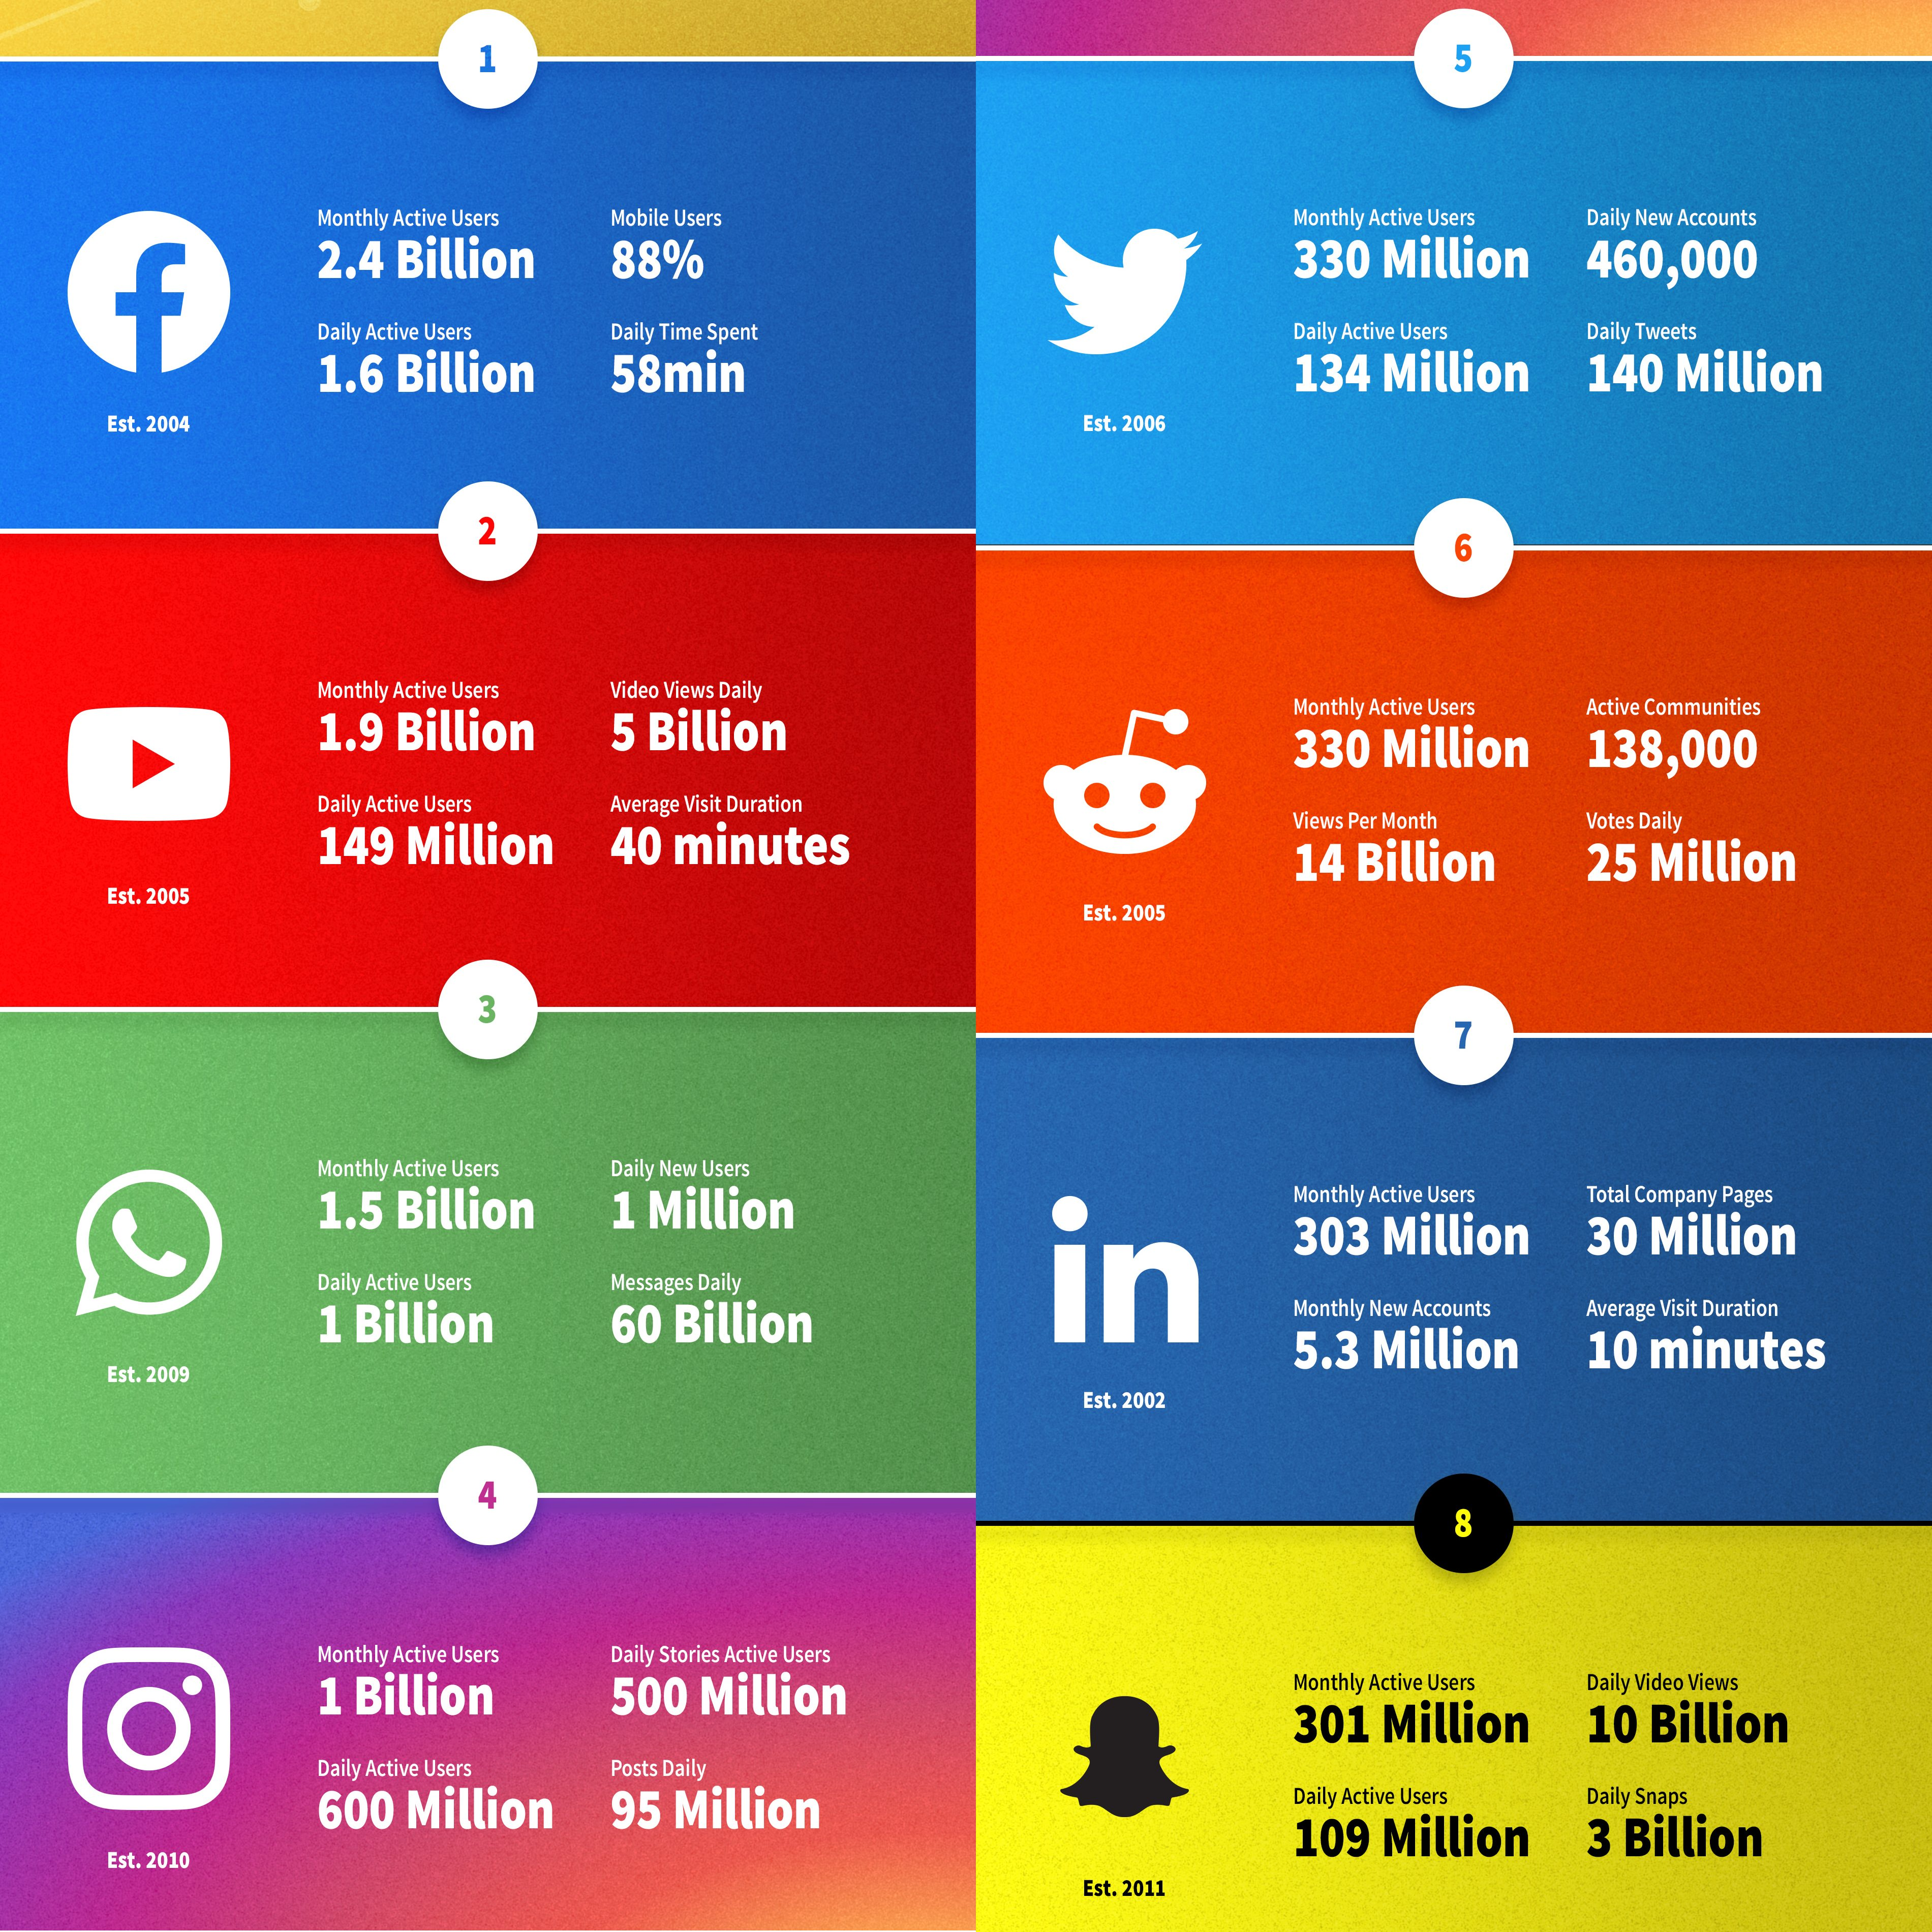
\includegraphics[width=0.8\linewidth]{img001.jpg}}\vspace{2mm}\\
	Source : https://dustinstout.com/social-media-statistics/
\end{center}

\newpage
\subsection{Les intervenants}

%\textit{Présenter ici une liste des intervenants non utilisateurs identifiés (un intervenant se distingue de l'utilisateur dans la mesure où il n'est pas en contact direct avec le système à réaliser).}

On considère l'équipe de développement elle-même (chef de projet, programmeurs, administrateur système) puis l’équipe d’évaluation externe (professeur, assistant, moniteur).


\begin{center}
	\begin{tabular}{|L{0.2\linewidth}|L{0.35\linewidth}|L{0.38\linewidth}|}
		\hline
		\textbf{Nom} & \textbf{Description} & \textbf{Rôle} \\
		\hline
%		\textit{Nommer le type d'intervenant.} & \textit{Décrire ce qu'il représente au regard du développement.} & \textit{Décrire les responsabilités et le rôle qu'il joue dans le développement, c'est-à-dire ses intérêts en tant qu'intervenant. Par exemple :
%		\begin{itemize}
%			\item S'assure qu'il y a une demande pour les fontionnalités
%			\item Contrôle l'avancement du projet
%			\item Approuve le budget
%			\item S'assure que le système sera maintenable
%			\item etc
%		\end{itemize}	
%		} \\
%		\hline
		\textbf{Chef de projet} & Il coordonne l’équipe de développement, tout en développant lui-même & Coordonner l’équipe, régler les bugs, gérer les disponibilités des membres de l’équipe \\
		\hline
		\textbf{Programmeur} & Il développe la plateforme & Maintenir le code, implémenter les fonctionnalités de la plateforme \\
		\hline
		\textbf{Administrateur système} & Il assure que le système (VM) soit fiable et le code de la plateforme soit fonctionnel. Il intègre le code en vérifiant la qualité du code (unit testing + system testing) & Assurer le bon fonctionnement du système, gérer les problèmes techniques, intégrer le code, exécuter les tests \\
		\hline
		\textbf{Équipe d’évaluation} & Professeur, assistant, moniteur (à définir) & Évalue la plateforme et ses fonctionnalités : Évaluer le code, utiliser l’interface de l’application, rédiger des rapports d’évaluation \\
		\hline
		\textbf{Législateur} & Propre à chaque pays, il possède le pouvoir de décider et faire appliquer les lois & Définit le cadre légal dans lequel Kernel doit opérer \\
		\hline
		\textbf{Régie publicitaire} & Offre des services publicitaires & Fournit la rémunération nécessaire à faire vivre Kernel \\
		\hline
	\end{tabular}
\end{center}

\subsection{Les utilisateurs}

%\textit{Présenter ici une liste des utilisateurs identifiés.}

On différencie les utilisateurs standards, premium et ceux souhaitant sponsoriser leurs publications.

\begin{center}
	\begin{tabular}{|C{0.18\hsize}|C{0.22\hsize}|C{0.25\hsize}|C{0.20\hsize}|}
		\hline
		\textbf{Nom} & \textbf{Description} & \textbf{Rôle} & \textbf{Représentant} \\
		\hline
%		\textit{Nommer le type d'utilisateur.} & \textit{Décrire leur lien avec le système à développer.} & \textit{Décrire le rôle qu'il  joue par rapport au système à développer (taches métier à automatiser, responsabilités dans le projet). Exemple :
%				\begin{itemize}
%					\item Récolter les détails d'une tache
%					\item Produire des rapports
%					\item Coordonner le travail
%				\end{itemize}	
%		} & \textit{Si l'utilisateur n'intervient pas directement, dire quel intervenant le représente tout au long du projet} \\
%		\hline
		\textbf{Utilisateurs standards} & Utiliser la plateforme de façon basique & Utiliser la plateforme avec des publicités et publications sponsorisées & Equipe d’évaluation, législateur \\
		\hline
		\textbf{Utilisateurs premium} & Bénéficie en plus de fonctionnalités avancées & Utiliser la plateforme sans publicités avec un fil d’actualité personalisé & Equipe d’évaluation, législateur \\
		\hline
		\textbf{Utilisateur (premium) sponsor} & Souhaite que ses publications soient visibles par d'autres utilisateurs & Paie pour des publications sponsorisées & Equipe d'évaluation, législateur \\
		\hline
	\end{tabular}
\end{center}

\subsection{Environnement utilisateur}

%\textit{Détailler l'environnement de travail de l'utilisateur final. Voici quelques suggestions :}
%\begin{itemize}
%	\item Nombre de personnes impliquées dans l'accomplissement d'une activité? Est-ce que cela va changer?
%	\item Quelle est la durée de chaque activité? Est-ce que cela va changer?
%	\item Y'a-t-il des contraintes spécifiques comme : environnement mobile, utilisation en extérieur ou dans un avion, sur un bateau, etc
%	\item Quelles sont les plateformes utilisées à l'heure actuelle? Les futures plate formes?
%	\item Quelles autres applications sont utilisées ? Est-ce que l'application à réaliser doit les intégrer ?
%\end{itemize}
	
%\textit{On peut ici inclure ou faire des références au Modèle Métier (Business Model) pour souligner une activité, l'implication des individus, etc}

Typiquement, les utilisateurs finaux utilisent des applications mobiles, ou parfois un navigateur internet, afin d’accéder à leurs réseaux sociaux. 

Kernel doit impérativement proposer une expérience similaire aux utilisateurs, donc permettre d’utiliser les fonctionnalités de base des réseaux sociaux dont ils ont l'habitude.




\subsection{Profils des intervenants}

\textit{Décrire chaque intervenant (non utilisateur) en remplissant les rubriques de la table ci-dessous}

\subsubsection{Chef de projet}

\begin{tabular}{|a|L{0.78\linewidth}|}
	\hline
	Représentant & Svetlana \\
	\hline
	Description & Membre de l'équipe de développement \\
	\hline
	Type & Novice-connaisseur en programmation, sans expertise en direction de projet \\
	\hline
	Responsabilités & Le chef de projet est particulièrement responsable de la performance de l'équipe et donc la réussite du projet \\
	\hline
	Critère de succès & Le projet arrive à un stade auquel il est utilisable et répond aux exigences listées dans ce document. La récompense pour le succès est la fierté d'accomplissement et l'obtention d'une bonne note. \\
	\hline
	Implications & Coordonne l’équipe de développement tout en développant, gére les disponibilités des membres de l’équipe. \\
	\hline
	Livrables & L'équipe de développement est bien organisée et peut travailler efficacement. \\
	\hline
	Comments/Issues & Si ce membre n'est pas efficace à son rôle, le reste de l'équipe et le projet en souffrira. \\
	\hline
\end{tabular}

\subsubsection{Programmeur}

\begin{tabular}{|a|L{0.78\linewidth}|}
\hline
Représentant & Tous les membres de l'équipe \\
\hline
Description & Membre de l'équipe de développement \\
\hline
Type & Novice-connaisseur en programmation, sans expertise dans ce type de projet \\
\hline
Responsabilités & Doit travailler en équipe et fournir du code de qualité \\
\hline
Critère de succès & Le projet arrive à un stade auquel il est utilisable et répond aux exigences listées dans ce document. La récompense pour le succès est la fierté d'accomplissement et l'obtention d'une bonne note. \\
\hline
Implications & Fait partie de l'équipe de développement \\
\hline
Livrables & Le code qui compose le projet (y compris les tests) et la documentation. \\
\hline
Comments/Issues & Si un membre n'est pas efficace à son rôle, le reste de l'équipe et le projet en souffrira. \\
\hline
\end{tabular}

\subsubsection{Administrateur Système}

\begin{tabular}{|a|L{0.78\linewidth}|}
\hline
Représentant & Mark \\
\hline
Description & Membre de l'équipe de développement \\
\hline
Type & Novice-connaisseur en programmation, sans expertise dans ce type de projet \\
\hline
Responsabilités & Assurer le bon fonctionnement du système (serveur et environnement de développement), gérer les problèmes techniques, intégrer le code, exécuter les tests \\
\hline
Critère de succès & Le projet arrive à un stade auquel il est utilisable et répond aux exigences listées dans ce document. La récompense pour le succès est la fierté d'accomplissement et l'obtention d'une bonne note. \\
\hline
Implications & Fait partie de l'équipe de développement et assume le rôle supplémentaire d'administrateur système. \\
\hline
Livrables & Les membres de l'équipe de développement ont les outils nécessaires  \\
\hline
Comments/Issues & Si un membre n'est pas efficace à son rôle, le reste de l'équipe et le projet en souffrira. \\
\hline
\end{tabular}


\subsection{Profils des utilisateurs}

%\textit{Décrire chaque utilisateur en remplissant la table ci-dessous. Les utilisateurs peuvent être des experts ou des novices. Ceci doit être reflété dans la description ci-dessous}

\subsubsection{Utilisateur standard}

\begin{tabular}{|a|L{0.7\linewidth}|}
	\hline
	Représentant & Équipe d'évaluation, législateur \\
	\hline
	Description & Utilisateur de réseaux sociaux, utilse gratuitement Kernel \\
	\hline
	Responsabilités & Respecter les règles d'utilisation, noter le service \\
	\hline
	Critère de succès & Le service répond à leur besoin, Kernel est plus agréable à utiliser que l'alternative. Possibilité de faire connaître sa satisfaction en note et commentaire. \\
	\hline
	Implications & Sans utilisateurs, Kernel n'est pas utile \\
	\hline
	Livrables & Retour (commentaire, note, etc) \\
	\hline
	Comments/Issues & Le large public peut avoir des attentes/goûts non envisagés, ou injustement mal noter le service \\
	\hline
\end{tabular}

\subsubsection{Utilisateur premium}

\begin{tabular}{|a|L{0.7\linewidth}|}
\hline
Représentant & Équipe d'évaluation, législateur \\
\hline
Description & Utilisateur de réseaux sociaux, utilse Kernel  de manière payante, souhaite une expérience avancée, sans publicité et avec accès au service de publications sponsorisées. \\
\hline
Responsabilités & Respecter les règles d'utilisation, noter le service \\
\hline
Critère de succès & Le service répond à leur besoin, Kernel est plus agréable à utiliser que l'alternative. Possibilité de faire connaître sa satisfaction en note et commentaire. \\
\hline
Implications & Sans ces utilisateurs, Kernel ne peut pas être rentable \\
\hline
Livrables & Retour (commentaire, note, etc) \\
\hline
Comments/Issues & Ce public peut avoir des attentes/goûts non envisagés, ou injustement mal noter le service \\
\hline
\end{tabular}

%\subsection{Besoins clés des intervenants et utilisateurs}
%
%\textit{Lister les besoins clés tels qu’ils sont perçus par l’intervenant ou l’utilisateur. Pour chaque besoin, clarifier les questions suivantes :
%\begin{itemize}
%	\item Quelles sont les causes du problème? 
%	\item Comment est-il résolu actuellement?
%	\item Quelles solutions l’intervenant veut-il?
%\end{itemize}
%Il est important de comprendre l’importance relative que l’intervenant attribue à la résolution de chaque problème. Le cumul des informations de tous les intervenants permet ensuite de définir des priorités de développement.  Pour ce faire, on peut s’aider du  tableau suivant.}
%
%\begin{center}
%	\begin{tabular}{|c|c|c|c|c|}
%	\hline
%	\textbf{Besoin (métier)} & \textbf{Priorité} & \textbf{Concerne} & \textbf{Solution actuelle} & \textbf{Solutions proposées} \\
%	\hline
%	&  &  &  &  \\
%	\hline
%\end{tabular}
%\end{center}


\subsection{Alternatives et concurrence}

%\textit{Identifier des alternatives que les intervenants jugent plausibles comme : achat, développement interne, évolution de système existant, conservation du status quo. Lister toutes les alternatives qui existent ou vont apparaitre Indiquer les forces et faiblesses principales de ces alternatives du point de vue des intervenants.}

\textbf{SocialHub}, \textbf{Buffer}, \textbf{Hootsuite}, \textbf{IM+}

Ces services sont similaires et partagent le fait qu'ils sont axés vers les entreprises et les individus importants.
\begin{itemize}
	\item Forces : Produit professionnel, clients bien définis, ressources, etc
	
	\item Faiblesse : Inaccessibles ou inintéressants pour le large public
\end{itemize}


\newpage
\section{Vue d'ensemble du produit}

%\textit{Cette section fournit une vue de haut niveau sur les propriétés et les caractéristiques du produit, les interfaces avec d’autres applications, et la configuration du système.}

\subsection{Perspective du produit}

%\textit{Présente le produit dans la perspectice des autres produits associés et de l’environnement utilisateur.Si le produit est un stand alone, il faut l’indiquer ici. S’il fait partie d’un système plus large, alors il faut indiquer comment ces systèmes interagissent et identifier lesinterfaces entre eux. Une bonne technique de documentation est d’utiliser un diagramme de blocs fonctionnels ou composants principaux avec leurs interfaces}

L'architecture de Kernel nécessite de s'appuyer sur les services externes (API) des réseaux sociaux, agissant comme \textit{intermédiaire} entre ceux-ci et l'utilisateur.

Le service de Kernel nécessite les composants basiques que sont : un client (ici une webapp, fonctionne sur le terminal de l'utilisateur), qui communique avec se(s) serveur(s) afin d'obtenir le contenu, et ce(s) serveur(s)  s'appuie(nt) sur une base de données (pour les information permanentes comme les informations sur l'utilisateur).

\vspace{4mm}
\begin{center}
	\fbox{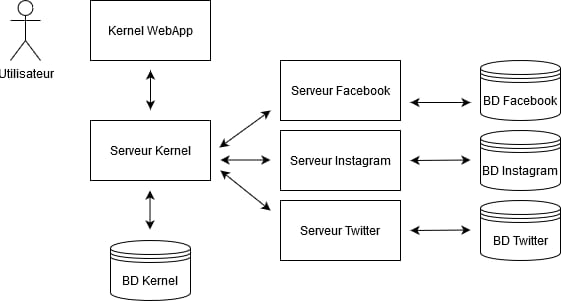
\includegraphics[width=0.65\linewidth]{img002}}
\end{center}

\subsection{Résumé des caractéristiques}

%\textit{Résumer les caractéristiques et avantages principaux que le système va fournir. Organiser les fonctionnalités de manière à ce qu’un utilisateur non technique ou n’importe quel lecteur non spécialiste puisse le comprendre. Par exemple, on peut utiliser une table présentant les avantages escomptés pour les futurs utilisateurs en termes très généraux, en les accompagnant des caractéristiques du produit qui rendent ces avantages possibles}

\begin{center}
	\begin{tabular}{|L{.25\textwidth}|L{.7\textwidth}|}
	\hline
	\textbf{Avantage pour l’utilisateur} & \textbf{Caractéristiques correspondantes} \\
%	\hline
%	\textit{Les clients mauvais payeurs sont identifiés} & \parbox{.5\linewidth}{\textit{Le système affiche à chaque entrée de commande une information sur le statut du client (normal, mauvais payeur)}} \\
	\hline
	Avoir un fil d'actualité \underline{unique} & L’application propose de regrouper les fils d’actualité en provenance des différents réseaux sociaux utilisés par l’utilisateur. \\
	\hline
	Présenter un fil d’actualité personalisé & L’application propose un fil d’actualité personalisé à l’utilisateur. \\
	\hline
	Gestion des publications & L’application propose de réaliser une même publication sur un ou plusieurs réseaux sociaux (au choix) parmi ceux utilisés. \\
	\hline
	Gestion des posts & L’application propose un filtrage des posts en provenance des différents réseaux sociaux selon les centre d’intérêts ou préférences des différents utilisateurs. \\
	\hline
	Présenter un seul fil de discussion par contact & L’application propose de regrouper les messages des différents contacts en provenance des différents réseaux sociaux en une messagerie unique. \\
	\hline
	Gérer un seul fil de discussion & L’application permet d’envoyer un message à un contact indépendamment du réseau social utilisé \\
	\hline
	Regrouper les contacts & L’application propose de regrouper les contacts en indiquant quels réseaux sociaux sont utilisés par chacun d’entre d’eux. \\
	\hline
	Etendre la notoriété & L’application permet de sponsoriser les contenus pour atteindre plus de personnes. \\
	\hline
	Etendre la notoriété & L’application facilite la présence sur de multiples réseaux sociaux. \\
	\hline
\end{tabular}
\end{center}


\subsection{Hypothèses}

%\textit{Lister chaque facteur pouvant affecter les caractéristiques du produit, en particulier  les éléments de l’environnement qui, s’is sont modifiées vont impliquer des modifications du document de vision. Par exemple, une hypothèse forte est la disponibilité dûn certain système d’exploitation, la disponibilité de données provenant de fournisseurs, la disponibilité d’une connexion internet, etc}

Les caractéristiques du service Kernel dépend des éléments suivante :
\begin{itemize}
	\item Accès aux APIs : Sans accès aux réseaux sociaux avec lesquels il doit intéragir, Kernel sera incapable de fonctionner. Il faudra se contenter des réseaux sociaux dont l'API répond à nos besoins.
	
	\item Temps : La contrainte de temps et la taille de l'équipe de développement borne sérieusement la quantité de fonctionnalités qui pourra être implémentée.
	
	\item Connaissance technique : Les domaines technique inconnus identifiés sont vastes et nombreux (et pas forcément aisés à apprendre), et notre expérience est très limitée, ce qui devrait grandement nous limiter en termes de sophistication.
	
	\item Technologies empruntées : Nous utilisons des technologies comme Docker, Kubernetes, Angular, etc, sans vraiment les comprendre entièrement, ce qui signifie que Kernel dépendra du bon fonctionnement de ces composantes externes. Nous dépendrons aussi du serveur et la connexion Internet de l'Université
\end{itemize}

\subsection{Coût et politique de prix}

%\textit{Indiquer les contraintes de cout et de pricing pertinentes pour le projet. Par exemple, on peut lister les couts de fabrication et de distribution des supports ou des manuels utilisateur. Déterminer aussi la politique de prix et le schema de pricing pour le produit. Cette rubrique peut être non pertinence dependant des projets, mais dans certains cas, elle peut influencer le développement.}

Bien qu'il fut déterminé que les comptes premium et les publications sponsorisées seraient payantes, nous n'avons pas d'idée fixe sur les coûts qui devraient y être associés pour le moment.

%\subsection{Licences et installation}
%
%\textit{Indiquer la politique de licence,  accompagnée des procédures d’installation. En effet cela peut avoir une influence sur le développement. Par exemple les dispositifs anti-piratage incluant une validation de la clé de produit via Internet impliquent des développements supplémentaires. Il s’agit aussi de tenir compte des éventuels scripts d’installation et produits associés requis.}






\section{Caractéristiques essentielles du produit}

%\textit{Lister et décrire brièvement les caractéristiques (features) essentielles du produit.Ce sont les fonctionnalités de haut niveau qui permettent d’apporter de la valeur ajoutée pour l’utilisateur. Par exemple, la possibilité de lister les clients mauvais payeurs (caractéristique) permet d’éviter les problèmes de facturation et de débiteur douteux (bénéfice). \\
%\\	
%Étant donné que le document de Vision est lu par une population  de personnes de niveau technique variable, la description doit se faire en termes suffisamment généraux pour que chacun puisse comprendre. Cette description sert de point d’entrée à la création du modèle des use-cases. Typiquement pour un nouveau système le nombre des caractéristiques est compris entre 25 et 100. Ces caractéristiques sont la base de la définition du produit final, de la définition de l’étendue du projet et de la gestion du projet. Chaque caractéristique va ensuite être détaillée dans le modèle des use-cases. Dans cette énumération des caractéristiques, éviter toute référence à la conception du système. On documente ici le "quoi" et le "pourquoi",  non pas le "comment".  }

\textcolor{blue}{En blue : \textbf{Must}}, en noir : \textbf{Should}, \textcolor{gray}{en gris : \textbf{Could}}



\begin{center}
	\begin{tabular}{|L{.25\textwidth}|L{.7\textwidth}|}
		\hline
		\textbf{Avantage pour l’utilisateur} & \textbf{Caractéristiques correspondantes} \\
%		\hline
%		\textit{Les clients mauvais payeurs sont identifiés} & \parbox{.5\linewidth}{\textit{Le système affiche à chaque entrée de commande une information sur le statut du client (normal, mauvais payeur)}} \\
		\hline
		\textcolor{blue}{Avoir un fil d'actualité \underline{unique}} & L’application propose de regrouper les fils d’actualité en provenance des différents réseaux sociaux utilisés par l’utilisateur. \\
		\hline
		Présenter un fil d’actualité personalisé & L’application propose un fil d’actualité personalisé à l’utilisateur. \\
		\hline
		\textcolor{blue}{Gestion des publications} & L’application propose de réaliser une même publication sur un ou plusieurs réseaux sociaux (au choix) parmi ceux utilisés. \\
		\hline
		\textcolor{gray}{Gestion des posts} & L’application propose un filtrage des posts en provenance des différents réseaux sociaux selon les centre d’intérêts ou préférences des différents utilisateurs. \\
		\hline
		\textcolor{blue}{Présenter un seul fil de discussion par contact} & L’application propose de regrouper les messages des différents contacts en provenance des différents réseaux sociaux en une messagerie unique. \\
		\hline
		Gérer un seul fil de discussion & L’application permet d’envoyer un message à un contact indépendamment du réseau social utilisé \\
		\hline
		Regrouper les contacts & L’application propose de regrouper les contacts en indiquant quels réseaux sociaux sont utilisés par chacun d’entre d’eux. \\
		\hline
		\textcolor{gray}{Etendre la notoriété} & L’application permet de sponsoriser les contenus pour atteindre plus de personnes. \\
		\hline
		Etendre la notoriété & L’application facilite la présence sur de multiples réseaux sociaux. \\
		\hline
	\end{tabular}
\end{center}


\newpage
\section{Contraintes sur le produit}

En plus des contraintes énoncées jusqu'ici (pricipalement en section 4.3), on peut mentionner :
\begin{itemize}
	\item Cadre légal : La législation de chaque pays doit être prise en compte car cela impose des limites sur ce que Kernel peut faire. En particulier, le \textbf{RGPD} devra être étudié.
	
	\item Capacité de test : La plupart des membres de l'équipe estiment ne pas faire partie de la population cible de Kernel. Il faudra donc se familiariser avec les réseaux sociaux et créer des comptes.
\end{itemize}


\section{Tolérances de qualité non fonctionnelles}

%\textit{Définir ici les tolerances de qualité globales pour les specifications non fonctionnelles telles que performance, robustesse, tolerance aux fautes, utilisabilité etc}

Voir le document joint \fbox{{\ttfamily Kernel\_NFR}}.




\section{Autres exigences sur le produit}

%\textit{A un haut niveau, liste des standards applicables, exigences de matériel ou de plate-forme, performance, et environnement.}
%
%\subsection{Standards applicables}
%
%\textit{Standards qui doivent être respectés par le produit}
%
\subsection{Besoins système}

Un serveur avec suffisamment de ressources (inclut mémoire de travail et de stockage, puissance de calcul et accès à internet), une plateforme de développement satisfaisante, des services externes fonctionnels, la non-annihilation de la population et des infrastructures (informez nous si vous avez lu ça).

%\subsection{Performance}
%
%\textit{Ceci inclut les facteurs de charge, de bande passante, temps de réponse, de fiabilité sous diverses conditions, etc}
%
%\subsection{Exigences liées à l'environnement}
%
%\textit{Pour des systèmes incluant du hardware, on pourra spécifier les exigences en termes de temperature, humidité, chocs, radiations,…Pour le software il s'agit plutôt de conditions d'utilisation, de disponibilité de ressources, de conditions de maintenance, de techniques de détection et correction d'erreurs}
%
%
\section{Exigence de documentation}
%
%\textit{Description des exigencies en matière de documentation papier, électronique et en ligne. Elle inclut l'utilisation de chartes graphiques, de logos ainsi que les prescription de longueur, de formattage d'impression etc}

Nous suivrons les directives quand aux exigeances de documentation imposées. Si non appliquable, nous adopterons une approche "just enough doc".

%
%\subsection{Manuel utilisateur}
%
%\subsection{Aide en ligne}
%
%\subsection{Guides d'installation et de configuration, fichier readme}
%
%\subsection{Packaging, labelling, copyright}
%
%\textit{Inclure les exigences par rapport à la présentation du conditionnement du produit, des écrans de démarrage, des notices de copyright, des logos à utiliser, des chartes graphiques, etc}

















\end{document}
